\documentclass[PICOReport.tex]{subfiles}

\begin{document}

\planck\ enabled an immense step forward in Galactic astrophysics~\citep{Planck2018:XII}. With seven full-sky polarization maps at frequencies between 30 and 353~GHz and a highest resolution of 5\arcmin, \planck\ provided entirely new and surprising data about the structure of the \ac{ISM}; the data have a lasting legacy for the foreseeable future. PICO will provide an even greater leap forward. It will produce 21 polarization maps of Galactic emission, and in the bands already probed by \planck\ they will be much deeper; for example, PICO's map at 321~GHz will be 105 times deeper than \planck's mean map depth at 353~GHz, and PICO's map at 30~GHz will be 17 times deeper than \planck's.  At 799~GHz PICO will have five times the resolution of \planck 's highest resolution map (Fig.~\ref{fig:allsky}). Such a data set can only be obtained from space. These data will complement a rich array of other polarization observations forthcoming in the next decade, including stellar polarization surveys to be combined with Gaia astrometry, and Faraday rotation measurements from  observations at radio wavelengths with the  Square Kilometer Array (SKA) and its precursors.
\begin{figure}[ht]
    \centering
    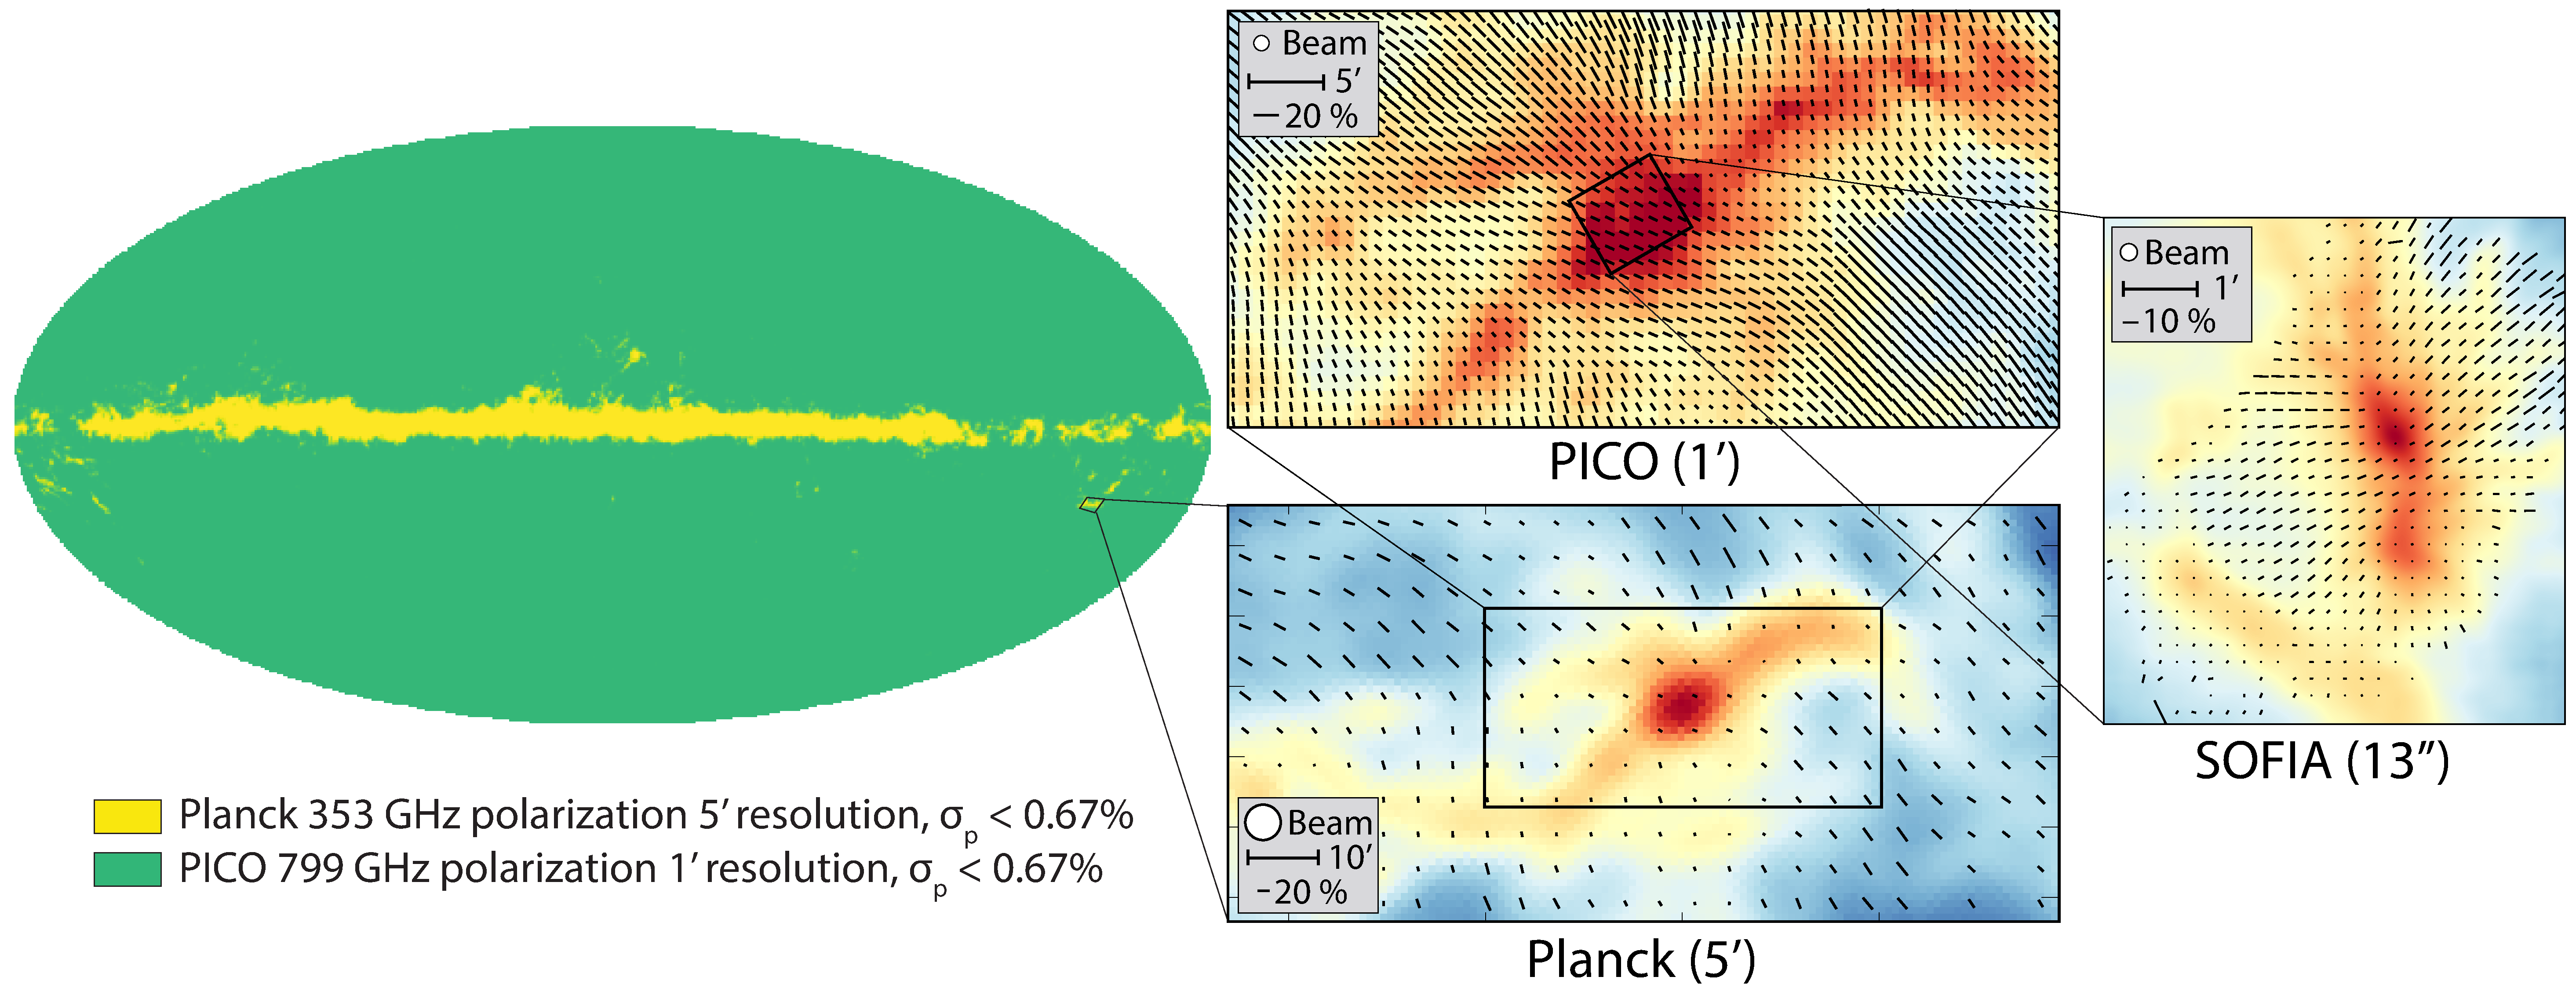
\includegraphics[width=6.5in]{galsci_fig_v4.pdf}
\vspace{-0.25in}
    \caption{\captiontext  \planck 's 353~GHz polarization map gave a resolution of 5\arcmin~and sensitivity to polarization intensity of $\sigma_{p} < 0.67\%$ over a small portion of the sky (left, yellow).  At 799 GHz, the PICO baseline mission will give a polarization map of the {\it entire sky} and with 5 times higher resolution (left, green). In the middle panels, the \planck~map of the Orion region overlaid with vectors that are aligned with the inferred magnetic field (lower panel), and a simulated PICO observation (upper panel) illustrate the leap in information content (vector lengths are proportional to polarization fraction). With this map, and maps at other frequencies, PICO will characterize Galactic magnetized turbulence at scales spanning the diffuse ISM down to dense star-forming cores, which will be mapped with high-resolution polarimetry by instruments such as HAWC+/SOFIA~\citep{Chuss2018} (right panel) and ALMA~\citep{Bacciotti2018ApJ}.
    \label{fig:allsky} }
\vspace{-0.10in}
\end{figure}

While the PICO data will likely provide many new insights and surprises, we focus here on two particularly important science objectives that are integral to NASA's science goal to explore how the Universe evolved; they relate to the structure and evolution of the Milky Way. These science objectives can only be achieved using the PICO dataset.

(1) {\em Test models of the composition of interstellar dust:} 
Less than $1\,\mu$m in size, dust grains are intermediate in the evolution from atoms and molecules to large solid bodies such as comets, asteroids, and planets. Encoded in the composition of dust are the pathways through which grains formed and grew. Dust grains also participate directly in interstellar chemistry, for example by catalyzing the formation of H$_2$ and organic molecules on their surfaces, in ways that depend upon their chemical makeup. Thus, the composition of dust grains is an essential aspect of the chemical evolution of interstellar matter, from the formation of complex molecules in space to the growth of planets. Through vastly improved spectral characterization of Galactic polarization, the PICO data will discriminate among models of Galactic dust composition to elucidate the chemical evolution of the Galaxy (SO6, \S~\ref{sec:test_composition_models}). The data will also guide the construction of methods for separating diffuse dust emission from cosmological signals of interest, particularly the inflationary signal. 
%\comor{can you please connect to 'galactic structure and evolution' (see example below)? also connect to foregrounds for B-mode if you think appropriate, or can leave this connection to later} \\

(2) {\em Determine how magnetic fields affect molecular cloud and star formation:}
Stars are formed through interactions between gravitational and magnetic fields, turbulence, and gas over more than four orders of magnitude of spatial scales, which span the diffuse ISM (kpc scale), molecular clouds (10~pc), and molecular cloud cores (0.1~pc). However, the role magnetic fields play in the large-scale structure of the diffuse \ac{ISM} and in the observed low star-formation efficiency has been elusive, owing to the dearth of data. By virtue of the strong dynamical coupling of dust and gas and the systematic alignment of dust grains with magnetic fields, PICO's dust polarization measurements will for the first time probe the large-scale Galactic magnetic field with enough resolution to trace the role of magnetic fields through the entirety of the star-formation process (SO7, \S~\ref{sec:magnetic_fields}). 


\subsubsection{Test Models of the Composition of Interstellar Dust}
\label{sec:test_composition_models}

Strong extinction features at 9.7~$\mu$m and 18~$\mu$m indicate that much of interstellar dust is in the form of amorphous silicates, while features at 217.5~nm, 3.3~$\mu$m, and 3.4~$\mu$m attest to abundant hydrocarbons. It is unknown, however, whether the silicate and carbonaceous materials coexist on the same grains or whether grains of each composition grow through distinct, parallel pathways dictated by their surface chemistry. 
%If there are indeed multiple grain populations, this will induce additional challenges for modeling the emission from interstellar dust in both total intensity and polarization at levels relevant for B-mode science at all angular scales~\citep{Hensley2018}. 

%\comor{The last sentence implies that the issue of multiple grain populations is only important for CMB B-mode science. Is it? Is it not important on its own right, because it is important to know what dust is made of? This is the missing connection to the broader picture: why do we care about dust?}

Some data suggest that the populations are distinct. Spectropolarimetry of dust extinction reveals robust polarization in the 9.7\,$\mu$m silicate feature~\citep{Smith2000}, indicating that the silicate grains are aligned with the interstellar magnetic field. In contrast, searches for polarization in the 3.4\,$\mu$m carbonaceous feature have yielded only upper limits, even along sightlines where silicate polarization is observed~\citep{Chiar2006,Mason2007}. These data are consistent with silicate and carbonaceous materials existing on separate grains that have different alignment properties. 
%\comblue{However, the 3.4~$\mu$m feature arises only from aliphatic (chain-like) carbonaceous material, which may not trace all carbon-bearing grains. Additionally, available data are restricted to only a few highly-extincted sightlines that may not typify the entire diffuse \ac{ISM}.}

At odds with the spectropolarimetric evidence from dust extinction are current measurements of the polarization fraction of the far-infrared dust emission with \planck~\citep{Planck_Int_XXII} and BLASTPol~\citep{Ashton2018}. They show little to no frequency dependence, whereas substantial frequency dependence would be expected if two components with distinct polarization properties were contributing to the total emission. 
%\comblue{However, current uncertainties are relatively large and the BLASTPol data are from only high density sightlines that may not be representative of the diffuse \ac{ISM}. }

With excellent polarization sensitivity, even in diffuse regions, PICO will provide a definitive test of the two-component paradigm \citep{Meisner2015}. 
%\comblue{To assess PICO's ability to discriminate models quantitatively, we employed the analytic two component dust model of Meisner et al.~\cite{Meisner2015}, which provided a better fit to IRAS and \planck\ data than one component models. We ran 1000 simulations with different combinations of polarization fractions of the two components. We used PICO baseline noise levels, frequency bands at and above 107~GHz, and binned the simulated data in 7.9$^\prime$ pixels, matching the beam of the PICO 107~GHz band.} 
In this case, the PICO baseline mission will determine the intrinsic polarization fractions of each of the two components to a precision of 3\%. With this level of precision the data will validate or reject state-of-the-art dust models~\citep[e.g.][]{Draine2009,Guillet2018}, test for the presence of additional grain species with distinct polarization signatures, such as magnetic nanoparticles~\citep{Draine2013}, and will be used as a crucial input for the foreground separation necessary to extract cosmological $E$- and $B$-mode science. 

Anomalous Microwave Emission (AME) is a component of Galactic emission peaking in the 20--30~GHz range that has been tentatively identified with small, rapidly-spinning dust grains~\citep{dickinson/etal:2018}. As only upper limits have been placed on its polarization, its role as a foreground for cosmological $B$-mode science remains unclear; even small levels of polarization could prove challenging for determining $r$~(\S~\ref{sec:signal_separation}). PICO will finely sample the AME SED with its bands at 21, 25, 30, 36, and 43 GHz. Combined with ground-based maps at lower frequencies, for example C-BASS at 5~GHz~\citep{Dickinson2018a}, PICO will be used to efficiently separate the AME from synchrotron and free-free emission and either detect or place stringent upper limits on its polarization. Further, the enhanced frequency coverage will allow changes in the AME SED with interstellar environment to be characterized and thus elucidate its underlying physics.

\subsubsection{Determine How Magnetic Fields Affect Molecular Cloud and Star Formation}
\label{sec:magnetic_fields}

Stars form out of dense, gravitationally unstable regions within molecular gas clouds, which themselves form through the flow of diffuse, atomic-phase gas to denser regions. Magnetic fields play an important role throughout this process. 

On the largest scales, magnetized turbulence mediates the flow of the gaseous \ac{ISM} from the atomic to the denser, molecular phase. Recent observations suggest that the structure of the diffuse medium is highly anisotropic, and strongly coupled to the local magnetic field~\citep{Clark:2014, Clark:2015, Kalberla:2016, KalberlaKerp:2016}. As molecular gas clouds collapse to form stars, magnetic fields can slow the process of star formation by inhibiting movement of gas in the direction perpendicular to the field lines. Observations to date suggest that the outer envelopes of clouds can be supported against gravity by magnetic fields and turbulence, but in dense cores gravity tends to dominate, and so these dense structures can collapse to form stars \citep{Crutcher2010}.  The degree to which magnetic fields affect the formation of molecular clouds, as well as stars within these clouds, is poorly constrained, in large part due to the difficulty of making detailed maps of magnetic fields in the ISM.

%Stars form out of dense, gravitationally unstable regions within molecular gas clouds. The efficiency of this conversion from molecular gas to stars is very low, due to regulation from supersonic turbulent gas motions, magnetic fields, and feedback from young stars \citep{McKee2007}.  Magnetic fields may play an important role in slowing the process of star formation by inhibiting movement of gas in the direction perpendicular to the field lines.  Observations to date suggest that the outer envelopes of clouds can be supported against gravity by magnetic fields and turbulence, but in dense cores gravity tends to dominate, and so these dense structures can collapse to form stars \citep{Crutcher2010}.

%On larger scales, the formation of gravitationally unstable clouds is regulated by the flow of diffuse material into the molecular phase\comor{(?)}, a process that is mediated by magnetized turbulence in the low-density \ac{ISM}. Structure formation in the diffuse \ac{ISM} is poorly understood, but as a precursor to star formation it is crucial to understand what drives molecular cloud formation. Recent observations suggest that the structure of the diffuse medium is highly anisotropic, and strongly coupled to the local magnetic field~\citep{Clark:2014, Clark:2015, Kalberla:2016, KalberlaKerp:2016}. However, the degree to which magnetic fields affect the formation of molecular clouds, as well as stars within these clouds, is poorly constrained, in large part due to the difficulty of making detailed maps of magnetic fields in the interstellar medium.

\noindent$\bullet$ {\bf Formation of Magnetized Molecular Clouds from the Diffuse Interstellar Medium} \hspace{0.1in}
A comprehensive understanding of the magnetized diffuse \ac{ISM} is challenging because of its diverse composition, its sheer expanse, and the multi-scale nature of the physics that shapes it. To understand how matter and energy are exchanged between the diffuse and dense media, it is essential to measure the properties of the magnetic field over more than four orders of magnitude in column density. PICO is unique in its ability to provide the necessary data. \textit{Planck} achieved measurements of the diffuse sky at 60\arcmin\ resolution, resulting in $\sim$30,000 independent measurements of the magnetic field direction.  With 1.1\arcmin~resolution PICO will expand the number of independent polarization measurements to 86,000,000~(Fig.~\ref{fig:allsky}). The data will thus robustly characterize turbulent properties like the Alfv\'{e}n Mach number, $\mathcal{M}_A$, across a previously unexplored regime of parameter space. 

PICO's observations will complement recently completed high-dynamic-range neutral hydrogen surveys, such as \HI4PI \citep{HI4PI:2016} and GALFA-\hi \citep{Peek:2018}, as well as planned surveys of interstellar gas, most prominently with the SKA and its pathfinders. One of the open questions in diffuse structure formation is how gas flows within and between phases of the \ac{ISM}. A planned all-sky absorption line survey with the forthcoming SKA-1 will increase the number of measurements of the \ac{ISM} gas temperature by several orders of magnitude~\citep{McClure-Griffiths2015}. Quantitative comparisons of the \ac{ISM} temperature distribution from SKA-1 and estimates of the magnetic field strength and coherence length scale from PICO will elucidate the role of magnetized turbulence in the flow of matter in the \ac{ISM} from diffuse regions to regions of denser molecular gas.

\noindent$\bullet$ {\bf Formation of Stars within Magnetized Molecular Clouds} \hspace{0.1in}
The role of the magnetic field in star formation is quantified by the ratio of the energies stored in magnetic and gravitational fields, and the ratio of the energy stored in the magnetic field to that stored in turbulence. The first ratio is parameterized through a mass-to-flux ratio $\mu$, and the second through $\mathcal{M}_A$. 

With full-sky coverage and a resolution of 1.1\arcmin, PICO will map all the molecular clouds out to a distance of 3.4\,kpc with better than 1\,pc resolution.  Extrapolating from the Bolocam Galactic Plane Survey \citep[BGPS,][]{EllsworthBowers2015}, PICO is expected to make highly detailed magnetic field maps of over 2,000 molecular clouds, with $10^3$--$10^5$  independent polarization measurements per cloud. These are the {\it only foreseeable} measurements that will give $\mu$ and $\mathcal{M}_A$ over a statistically significant sample of molecular clouds. \planck , for example, mapped only ten nearby clouds to a similar level of detail~\citep{Planck:XXXV}. A large sample of clouds is crucial because: (1)~dust polarization observations are sensitive only to the magnetic field projected on the plane of the sky, and therefore polarization maps will look very different for molecular clouds observed at different viewing angles; and (2)~the relative importance of the magnetic field will likely be a function of cloud age and mass. By observing thousands of molecular clouds PICO will determine $\mu$ and  $\mathcal{M}_A$ for different sub-classes of cloud age and mass. 

\subsubsection{Galactic Legacy Science}
\label{sec:galactic_legacy}

PICO will also produce legacy datasets that will revolutionize our understanding of how magnetic fields influence physical processes ranging from planet formation to galaxy evolution.  For ten clouds closer than 500 pc, PICO will resolve magnetic fields on scales of 0.1~pc. This is the scale of dense cores and filaments for these clouds, and thus the observations will constrain how magnetic fields on these scales influence the formation of cloud cores.  Currently no experiment has the sensitivity and resolution to observe both the the large-scale (few parsec) and core-scale magnetic fields. By comparing the orientation of the core-scale magnetic fields with the orientation and sizes of proto-planetary disks, PICO will probe whether magnetic braking influences the growth of such disks~\citep{allen_2003,li_2014} and provide complementarity to higher angular resolution instruments such as ALMA and SOFIA~\citep{Bacciotti2018ApJ,Harper2018}~(Fig.~\ref{fig:allsky}).
%\comor{isn't ALMA or other instruments better suited for this?}

Key processes in the diffuse ISM, including heat transport, streaming of cosmic rays, and magnetic reconnection depend strongly on the level of the environment's magnetization~\citep{Lazarian:2006,Lazarian:2016,Lazarian_Vishniac:1999}.
PICO will give information about these processes with tens of millions of independent measurements of magnetic field orientation over the entire Galaxy. The measurements will also enable studies of the physical processes that generate magnetic fields through a combination of turbulence and large-scale gas motions~\citep{Xu_2018}.

Finally, PICO observations will create detailed magnetic field maps of about 70 nearby galaxies, with 100 or more measurements of magnetic field directions per galaxy. Currently, polarized dust emission has only been observed in M82 and NGC 253 using SOFIA~\citep{Jonesetal}. The PICO observations will determine how interaction between large-scale magnetic fields, turbulence, and feedback from previous generations of star formation affect galaxy evolution and star-formation efficiency.

\end{document}

%\begin{figure}[!htb]
%\centering
%
\includegraphics[width=4cm]{images/example}
%\caption{example}
%\label{fig:im_3}
%\end{figure}
